\chapter{One-Variable Equation}

There are variety of ways to solve the scalar function $f(x)=0$ for scalar independent variable $x$, the most intuitive of which being deriving its analytical solution in the explicit form. However, in many cases the explicit analytical solution of $x$ may not be achievable due to the complexity of $f(x)$. To address this problem, many numerical analysis based methods have been developed to obtain (an approximation of) the solution effectively and efficiently.

This chapter discusses these numerical methods as well as their convergence and computational burden.

It is worth mentioning that many methods introduced in this chapter, such as Newton's method, can be easily expanded to solve vector functions with vector independent variables. Nevertheless, for the convenience of the illustration, only scalar function with scalar input is considered in this chapter.

\section{General Problem Formulation}

Let $f(x)=0$ be a scalar function, where $f(x)$ is continuous. There is at least one solution to $f(x)=0$, namely $p$, and $p\in \left[a, b\right]$. The target is to find $p$. A demonstrative plot is given in Fig. \ref{fig:part-5:onevarproblemformulation}. In the example, function $f(x)=0$ has two solutions within $\left[0, 10\right]$. The target is to find any one of them.

\begin{figure}[!htbp]
\centering
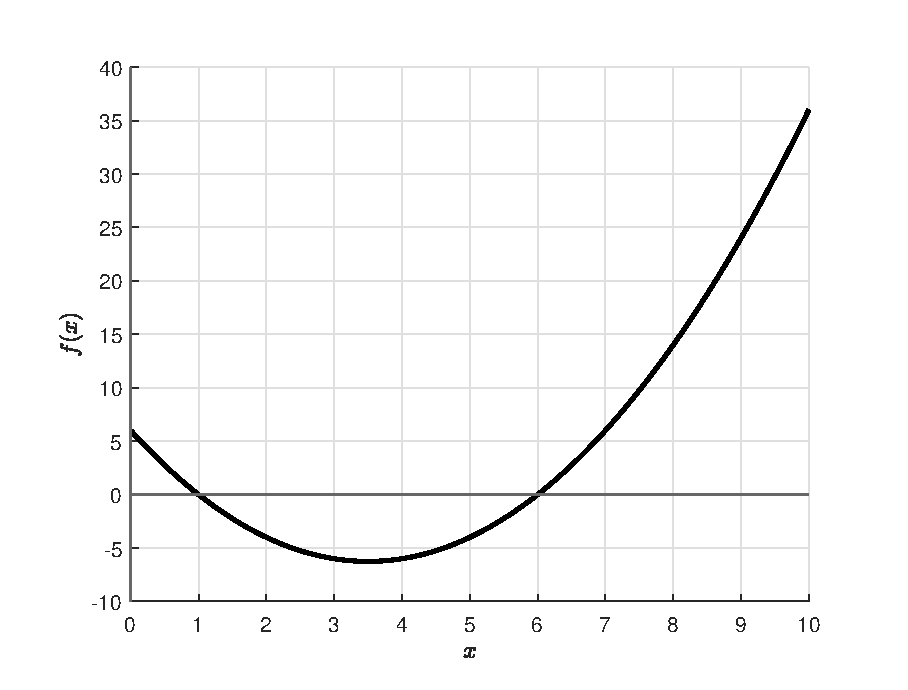
\includegraphics[width=250pt]{chapters/part-5/figures/demo_problem_formulation.eps}
\caption{A demonstrative example of solving $f(x)=0$ using numerical methods.} \label{fig:part-5:onevarproblemformulation}
\end{figure} 

Notice that there might be other solutions to $f(x)=0$ within $\left[a, b\right]$ than $p$. Useful it may be to find all solutions, however, in the scope of our discussion we look for only one solution. 

\section{Solution}

A scalar function can be solved numerically via the following methods, each with some pros and cons.

\subsection{Bisection Method}

Bisection method, also known as the binary search method, is inspired by the \textit{intermediate value theorem}. So long as we can find an interval $\left[a, b\right]$ so that $f(a)f(b)<0$, we know that there must be such a solution $p\in\left[a, b\right]$ that $f(p)=0$. If we can narrow down the interval, we can approach the solution.

\begin{shortbox}
\Boxhead{Intermediate Value Theorem}

Let $f(x)$ be a continuous function whose domain contains the interval $\left[a, b\right]$. Without loosing generality, let us assume that $f(a)<f(b)$. Then $\forall c \in \left[f(a), f(b)\right]$, $\exists x_0 \in \left[a, b\right]$, so that $f(x_0)=c$.

\end{shortbox}

The algorithm is summarized as follows. Let $f(x)$ be a continuous function on $\left[a, b\right]$, and $f(a)f(b)<0$. Do the following to find a solution $f(p)=0$ within $\left[a, b\right]$.

\begin{enumerate}
\item Let $a_1 = a$, $b_1=b$.
\item Let $p_i = \frac{a_i+b_i}{2}$.
\item Calculate $f(p_i)$. If $f(p_i)=0$, then $p_i$ is a solution. Otherwise:
\begin{itemize}
  \item If $f(p_i)f(a_i) < 0$, let $a_{i+1}=a_i, b_{i+1}=p_i$.
  \item If $f(p_i)f(b_i) < 0$, let $a_{i+1}=p_i, b_{i+1}=b_i$.
\end{itemize}
\item Check stop criteria as follows:
\begin{itemize}
  \item If the solution $p_i$ is found, return $p_i$;
  \item If the interval $b_{i+1}-a_{i+1}$ is less than a threshold, return either $a_{i+1}$ or $b_{i+1}$;
  \item If the number of iteration exceeds the maximum iteration limit, return either $a_{i+1}$ or $b_{i+1}$ together with a warning flag;
  \item Otherwise, iterate from Step 2. 
\end{itemize}
\end{enumerate}

Bisection method is intuitive and it can definitely find the solution. The down side of the method is that it takes many iterations to converge, hence not very efficient.

\subsection{Fixed Point Iteration Method}

A \textit{fixed point} of a function $f(x)$ is such $x=x_0$ that $f(x_0)=x_0$. The problem of solving an equation can be converted into finding a fixed point of a function. Consider solving $f(x)=0$ for its solution $p$. Let
\begin{eqnarray}
  g(x) &=& x + af(x) \label{eq:fixedpoint_p}
\end{eqnarray}
where $a\neq 0$ can be any value we choose, for example $a=1$. Clearly, a fixed point $p$ of $g(x)$ must be a solution to $f(x)$ because $g(p)=p$ according to the definition and substituting it into \eqref{eq:fixedpoint_p} gives
\begin{eqnarray}
  p &=& p + af(p)
\end{eqnarray}
hence $f(p)=0$ for $a\neq 0$.

The remaining of this section discusses when the fixed point exists and how to find one.

Fixed points of a function can be easily identified in the plot. A fixed point of $g(x)$ is its intersection with $y=x$ as shown in Fig. \ref{fig:part-5:fixed_point}. Function $g(x)=x^2-2$ is given by the solid line and $y=x$ the dashed line. Their two intersections, $p_1=-1$ and $p_2=2$, are the fixed point of $g(x)$.

\begin{figure}[!htbp]
\centering
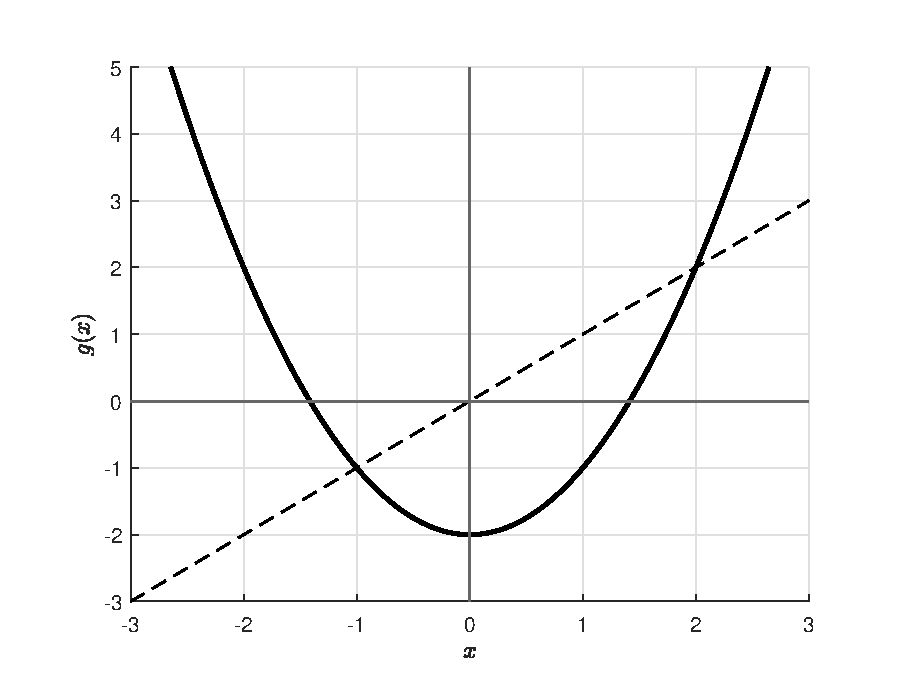
\includegraphics[width=250pt]{chapters/part-5/figures/demo_fixed_point.eps}
\caption{Function $g(x)=x^2-2$ and its two fixed points, $p_1=-1$ and $p_2=2$.} \label{fig:part-5:fixed_point}
\end{figure}

The following criterion can be used to find an interval for a fixed point: 
\begin{itemize}
  \item For continuous function $g(x)$, if for an interval $[a, b]$, $\forall x \in [a, b]$, $g(x)\in [a, b]$, then there is at least one fixed point of $g(x)$ in interval $[a, b]$.
  \item Furthermore, if the derivative $g\textprime(x)$ exists in $(a, b)$ and $\forall x \in (a, b)$, $|g\textprime(x)|<1$, then the fixed point is unique.
\end{itemize}
The proof is fairly straight forward and are not given here.

The fixed point of a function might be found via fixed point iteration. The idea is to use a series $\{p_n\}$ to approximate the fixed point $p$ with $n\rightarrow\infty$. The steps are summarized below.
\begin{enumerate}
  \item Select $p_1\in[a, b]$
  \item Calculate $p_{i+1} = g(p_i)$
  \item Check stop criteria as follows:
  \begin{itemize}
    \item If $p_{i+1}-p_i$ is less than a threshold, return $p_{i+1}$;
    \item If the number of iteration exceeds the maximum iteration limit, return $p_{i+1}$ together with a warning flag;
    \item Otherwise, iterate from step 2.
  \end{itemize}
\end{enumerate}

This method is illustrated in Fig. \ref{fig:part-5:fixed_point_iteration}. It can be seen from the figure how series $\{p_n\}$ approaches the fixed point $p$.

\begin{figure}[!htbp]
\centering
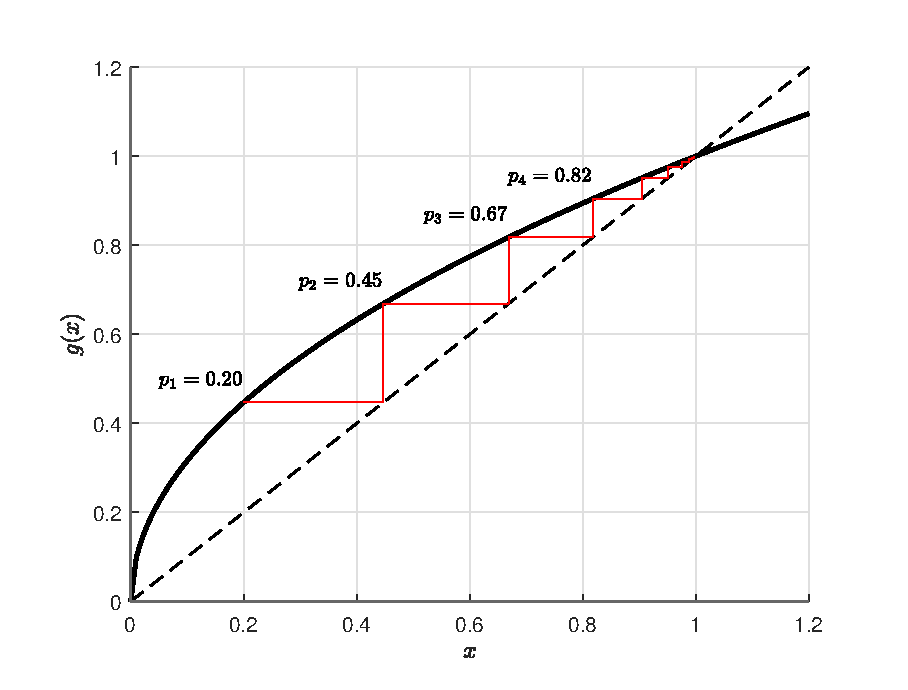
\includegraphics[width=250pt]{chapters/part-5/figures/demo_fixed_point_iteration.eps}
\caption{Approaching fixed point using fixed point iteration.} \label{fig:part-5:fixed_point_iteration}
\end{figure}

Notice that unlike bisection method, the aforementioned fixed point iteration method does not necessarily converge, and the key is the gradient $|g\textprime(x)|$ within the interval $(a, b)$. To be more precise,
\begin{itemize}
  \item If for $g(x)$ defined in interval $[a, b]$, if $g(x)\in[a, b]$ and $|g\textprime(x)|<1$ in $(a, b)$, then the aforementioned fixed point iteration method converges.
\end{itemize}
and this can be interpreted easily from a plot like Fig. \ref{fig:part-5:fixed_point_iteration}.

\subsection{Newton's method}

Newton's method, or Newton-Raphson method, is one of the most popular methods to solve equations numerically. It is intuitive and in most applications it converges fairly easily and fast. Broadly speaking, Newton's method is a special case of the fixed point iteration as it also construct a series $\{p_n\}$ that approaches to the solution of $f(x)=0$. Unlike \eqref{eq:fixedpoint_p}, the series looks like
\begin{eqnarray}
  g(x) &=& x - \frac{f(x)}{f\textprime(x)} \label{eq:newtonmethod}
\end{eqnarray}
given that $f\textprime(x)\neq 0$ in the concerned interval $(a,b)$. A fixed point of \eqref{eq:newtonmethod}, i.e. $g(p)=p$, obviously satisfies $f(p)=0$ and it can be proved by substituting $g(p)=p$ into \eqref{eq:newtonmethod}.

From \eqref{eq:newtonmethod}, consider constructing the series as follows
\begin{eqnarray}
  p_{i+1} &=& p_i - \frac{f(p_i)}{f\textprime(p_i)} \label{eq:newtonmethod_series}
\end{eqnarray}
Newton's method iterates \eqref{eq:newtonmethod_series} to approach the solution. A demonstrative Fig. \ref{fig:part-5:newton} is given below.
\begin{figure}[!htbp]
\centering
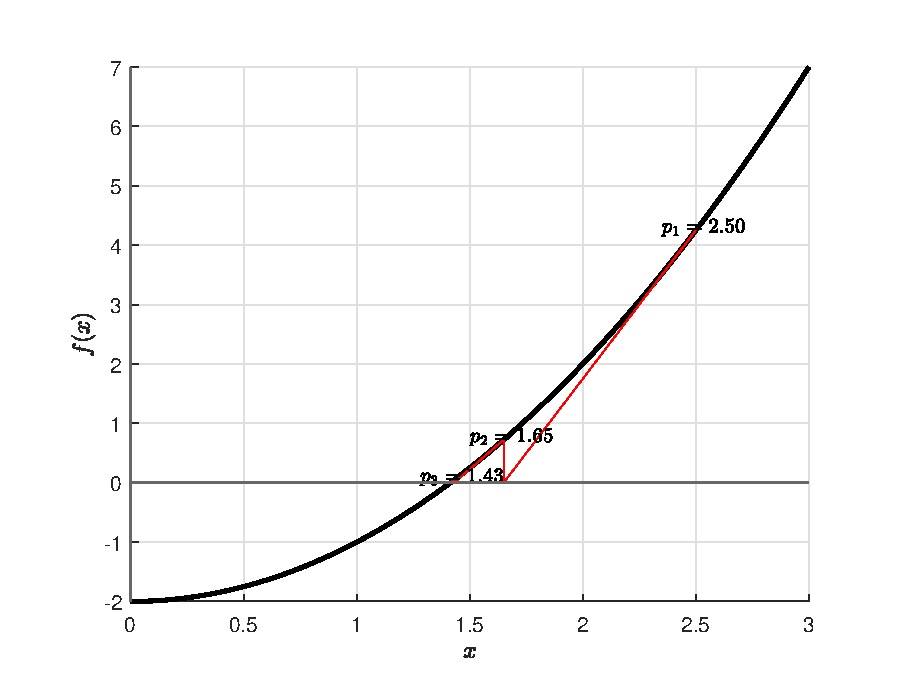
\includegraphics[width=250pt]{chapters/part-5/figures/demo_newton.eps}
\caption{A demonstration of using Newton's method to solve an equation.} \label{fig:part-5:newton}
\end{figure}
It can be seen from Fig. \ref{fig:part-5:newton} that in this example the iteration in \eqref{eq:newtonmethod_series} quickly converges the solution by tracing the gradient of $f(x)$. 

Indeed, with the same number of iterations, Newton's method usually gets to the solution faster than the bisection and the conventional fixed point iteration methods. The more ``linear'' $f(x)$ is around the solution, the faster and more accurately Newton's method would converge. As long as $f\textprime(x)\neq 0$ at the solution, there is always a neighbourhood around the solution where Newton's method converges. 

The only drawback of Newton's method, comparing with the other methods introduced so far, is that it requires the calculation of $f\textprime(x)$ in the iteration. This may not be a big issue if $f\textprime(x)$ can be calculated easily (for example, when its analytical form is available), but it may pose a problem if this is not the case.

\subsection{Secant Method}

The secant method might be used as an alternative to the Newton's method. Instead of \eqref{eq:newtonmethod_series}, the secant method uses the following series
\begin{eqnarray}
  p_{i+1} &=& p_i - \frac{f(p_i)(p_i-p_{i-1})}{f(p_i)-f(p_{i-1})} \nonumber
\end{eqnarray}
with two closed initial guesses $p_1$ and $p_2$ in the interval. The idea behind secant method is simple: it uses the secant of two consecutive samples, $p_i$ and $p_{i-1}$, to approximate the gradient $f\textprime(p_i)$.

The secant method is a little bit slower than the Newton's method in terms of convergence. Yet, it can be useful when $f(x)$ is significantly easier to calculate than $f\textprime(x)$.

\subsection{Muller's Method}

Muller's method is an extension to the secant method. Recall in the secant method, two initial points $p_1$ and $p_2$ are selected as the initial samples. In the essence, it fits a first-order polynomial $P(x)=ax+b$ that passes through $p_1, f(p_1)$ and $(p_2, f(p_2))$. The value of $a, b$ can be calibrated and the solution to $P(x)=0$ can be calculated analytically, which gives $p_3$. If $f(p_3)=0$, it returns the solution. Otherwise, it iterate the process with $(p_2, f(p_2))$ and $(p_3, f(p_3))$ now becoming the new samples to form the first-order polynomial.

Instead of using first-order polynomial $P(x)=ax + b$ to approximate the original function $f(x)$ near its solution, Muller's method uses second-order polynomial $P(x)=ax^2+bx+c$ for the same trick. To calibrate the parameters, three samples, $p_1$, $p_2$ and $p_3$ are required instead of two samples in the case of the secant method.

\section{Convergence Speed and Error}

The convergency of the methods introduced earlier have been briefly discussed in the previous section. This section digs deeper into the convergency criteria and speed of the methods, and performs error analysis to the methods. New algorithms will be proposed on top of the methods to improve them.

\subsection{Order of Convergence}

Let $\{p_n\}$ be a series that converges to $p$. To measure the speed of convergence of the series, define the order of convergence $\alpha$ and the asymptotic error constant $\lambda$ as follows.
\begin{eqnarray}
  \lim_{i\rightarrow\infty} \frac{|p_{i+1}-p|}{|p_i-p|^\alpha} &=& \lambda \label{eq:series_convergence_speed}
\end{eqnarray}
In \eqref{eq:series_convergence_speed}, the larger the value of $\alpha$, the faster the convergence. When $\alpha=1$ and $\lambda < 1$, the series is called linear convergence. When $\alpha=2$ and $\alpha=3$, the series is called quadratic convergence and cubic convergence, respectively. With everything otherwise the same, we usually prefer a series with a higher order of convergence when using it in the fixed point iteration.

Let $g$ be the recurrence relation of series $\{p_n\}$, i.e., $p_{i+1} = g(p_i)$. The series converges to $p$. The following statements are true. The proof is not given in this notebook.
\begin{itemize}
  \item If $g\textprime(p)\neq0$, then $\{p_n\}$ is linear convergence with asymptotic error constant $|g\textprime(p)|$.
  \item If $g\textprime(p)=0$, then there is a neighbourhood of $p$ where $\{p_n\}$ is at least quadratic convergence. Furthermore, let the upper bound $|g\textprime\textprime(p)| < M$, then
  \begin{eqnarray}
  \lim_{i\rightarrow\infty} \frac{|p_{i+1}-p|}{|p_i-p|^2} &<& \frac{M}{2} \nonumber
\end{eqnarray}
\end{itemize} 


From \eqref{eq:fixedpoint_p} and \eqref{eq:newtonmethod}, we know that while the conventional fixed point iteration is linear convergence, the Newton's method is at least quadratic convergence. This explains why Newton's method converges faster than the conventional fixed point iteration.

\subsection{Multiple Root}

When the original equation $f(x)=0$ has multiple roots at $x=p$, i.e.,
\begin{eqnarray}
  f(x) &=& (x-p)^mq(x) \nonumber
\end{eqnarray}
with $\lim_{x\rightarrow p} \neq 0$ and $m\geq 2$, the methods introduced so far may not work efficiently.

The multiple roots at $x=p$ can be observed by checking the gradient $f\textprime(x)$ at $p$. We can prove that
\begin{itemize}
  \item For a continuous function $f(x)$ defined in $[a, b]$, $p\in(a,b)$ is its single root if and only if $f(p)=0$ and $f\textprime(p)\neq 0$.
  \item For a continuous function $f(x)$ defined in $[a, b]$, $p\in(a,b)$ is its $m$ multiple roots if and only if $0=f(p)=f\textprime(p)=...=f^{(m-1)}(p)$ and $f^{(m)}(p)\neq 0$.
\end{itemize}

For Newton's method, on may notice from Fig. \ref{fig:part-5:newton} that if there are multiple roots and $f\textprime(p)=0$ at the solution, though Newton's method still converges, the convergence may slow down. The intuition is indeed correct. Newton's method is usually quadratic convergence when $f\textprime(p)\neq 0$. However, when $f\textprime(p)=0$, it may not be the case.

If an equation $f(x)=(x-p)^mq(x)$ has $m$ multiple roots at $p$, one way to handle it is to define
\begin{eqnarray}
  \mu(x) &=& \frac{f(x)}{f\textprime (x)} \nonumber
\end{eqnarray}
where it can be proved that $\mu(x)$ has a single root at $x=p$. Then, apply Newton's method on $\mu(x)$ to get the solution $p$. 

\subsection{Convergence Acceleration}

Aitken $\Delta^2$ method is used to form a new series $\{\hat{p}_n\}$ based on a linear convergent series $\{p_n\}$, where both series converges to $p$ but $\{\hat{p}_n\}$ converges faster. 

Aitken $\Delta^2$ method defines
\begin{eqnarray}
  \hat{p}_i &=& p_i - \frac{(p_{i+1}-p_i)^2}{p_{i+2}-2p_{i+1}+p_i} \nonumber
\end{eqnarray}
The idea is to calculate $p_i$ normally, and while doing that also calculate $\hat{p}_i$ using $p_i$, $p_{i+1}$ and $p_{i+2}$.

Aitken $\Delta^2$ method can be used to accelerate fixed point iteration. The idea is as follows.
\begin{enumerate}
  \item Calculate $p_1$, $p_2=g(p_1)$ and $p_3=g(p_2)$ normally.
  \item Calculate $\hat{p}_1$ using $p_1$, $p_2$ and $p_3$.
  \item Overwrite $p_1$ with $\hat{p}_1$, and repeat from Step 1.
\end{enumerate}
and it is known as the Steffensen method.

\section{Root for Polynomial}

Polynomial is a special type of a function that looks like
\begin{eqnarray}
  f(x) &=& a_nx^n + a_{n-1}x^{n-1} + \ldots + a_1x + a_0 \nonumber
\end{eqnarray}
where $a_n \in \mathbb{R}$ and $a_n\neq 0$. Variable $n$ is known as the order of the polynomial. In this case, $f(x)$ is often denoted as $P(x)$. Notice that $P(x)=0$ by concept is also a polynomial with no order, but it is often not an interest of study. For the remaining, we will only look at polynomials with $n\geq 1$. 

It can be proved (requiring theory from complex analysis) that:
\begin{itemize}
  \item Polynomial equation $P(x)=0$ with $n\geq 1$ has at least one root. The root can be real number or complex number.
  \item Polynomial equation $P(x)=n$ with the order of $n$ can be uniquely decomposed into the following form:
  \begin{eqnarray}
  P(x) &=& a_n(x-x_1)^{m_1}(x-x_2)^{m_2}\ldots(x-x_k)^{m_k} \nonumber
\end{eqnarray}
where $\sum m_i = n$, and $x_i$ being its $m_i$ multiple root.
  \item For two polynomials both less or equal to $n$th order, $P(x)$ and $Q(x)$, if there are distinct values $x_1, x_2, ..., x_k$ where $P(x_i)=Q(x_i)$, $i = 1,...,k$, and $k>n$, then $P(x)=Q(x)$ $\forall x$.
\end{itemize}

Finding the numerical solution for a general equation $f(x)=0$ using different methods, such as the Newton's method, has been introduced in earlier sections. When comes to polynomial equation $P(x)=0$, we can further improve the algorithms for better computation efficiency.

Given a polynomial $P(x)$ and a specified variable $x_0$, $P(x)$ can be decomposed as follows
\begin{eqnarray}
P(x) &=& (x-x_0)Q(x) + b_0 \label{eq:hornermethod}
\end{eqnarray}
where
\begin{eqnarray}
  Q(x) &=& b_nx^{n-1} + b_{n-1}x^{n-2} + \ldots + b_2x + b_1 \nonumber \\
  b_n &=& a_n \nonumber \\
  b_k &=& a_k + b_{k+1}x_0, k=n-1, n-2, \ldots, 1, 0 \nonumber
\end{eqnarray}
The proof is brute-force and are neglected here.

Obviously, from \eqref{eq:hornermethod} $b_0 = P(x_0)$. The decomposition provides an efficient way to calculate $P(x_0)$, which is usually faster than substituting $x_0$ into $P(x)$ directly and calculate $a_ix^i$ for all the terms. Furthermore, we know from \eqref{eq:hornermethod} that $P\textprime(x_0)=Q(x_0)$. This helps with speeding up the Newton's method to solve $P(x)=0$. This is known as the Horner method.



